%%%%%%%%%%%%%%%%%%%%%%%%%%%%%%%%%%%%%%%%%%%%%%%
% University Paderborn Beamer Presentation 

% Author: Ashwin Prasad Shivarpatna Venkatesh 

%This template is free: you can redistribute it and/or modify
%it under the terms of the GNU General Public License as published by
%the Free Software Foundation, either version 3 of the License, or any later version.
%
%This program is distributed in the hope that it will be useful,
%but WITHOUT ANY WARRANTY; without even the implied warranty of
%MERCHANTABILITY or FITNESS FOR A PARTICULAR PURPOSE.  See the
%GNU General Public License for more details.
%
%You should have received a copy of the GNU General Public License
%along with this program.  If not, see <https://www.gnu.org/licenses/>.

%%%%%%%%%%%%%%%%%%%%%%%%%%%%%%%%%%%%%%%%%%%%%%%

\documentclass{beamer}
% Default page size 12.8cm x 9.6cm

% import packages and user-defined commands
\usepackage{graphicx} % Allows including images
\usepackage{booktabs} % Allows the use of \toprule, \midrule and \bottomrule in tables
\usepackage{tikz}

\usepackage{helvet} % Font

\usepackage[english]{babel}
\usepackage{textcomp}
\usepackage{helvet} % Font
\usepackage{array}
\usepackage{listings}
\usepackage{color}
%\usepackage{lstlinebgrd} % install this package manually to enable line highlighting in lslisting
\usepackage{tikz}
\usetikzlibrary{shadows}
\definecolor{mygreen}{rgb}{0,0.6,0}
\definecolor{dkgreen}{rgb}{0,0.6,0}
\definecolor{gray}{rgb}{0.5,0.5,0.5}
\definecolor{mygray}{rgb}{0.5,0.5,0.5}
\definecolor{mymauve}{rgb}{0.58,0,0.82}

\lstset{ %
	language=[x86masm]Assembler,       % the language of the code
	basicstyle=\footnotesize,       % the size of the fonts that are used for the code
	numbers=left,                   % where to put the line-numbers
	numberstyle=\tiny\color{gray},  % the style that is used for the line-numbers
	stepnumber=1,                   % the step between two line-numbers. If it's 1, each line 
	% will be numbered
	numbersep=5pt,                  % how far the line-numbers are from the code
	backgroundcolor=\color{white},  % choose the background color. You must add \usepackage{color}
	showspaces=false,               % show spaces adding particular underscores
	showstringspaces=false,         % underline spaces within strings
	showtabs=false,                 % show tabs within strings adding particular underscores
	frame=single,                   % adds a frame around the code
	rulecolor=\color{black},        % if not set, the frame-color may be changed on line-breaks within not-black text (e.g. commens (green here))
	tabsize=2,                      % sets default tabsize to 2 spaces
	captionpos=b,                   % sets the caption-position to bottom
	breaklines=true,                % sets automatic line breaking
	breakatwhitespace=false,        % sets if automatic breaks should only happen at whitespace
	title=\lstname,                 % show the filename of files included with \lstinputlisting;
	% also try caption instead of title
	keywordstyle=\color{blue},          % keyword style
	commentstyle=\color{dkgreen},       % comment style
	stringstyle=\color{mauve},         % string literal style
	escapeinside={\%*}{*)},            % if you want to add a comment within your code
	morekeywords={*,...}               % if you want to add more keywords to the set
}

\newcommand*{\upblogo}{
\includegraphics[width=3cm]{logo.pdf}}
\newcommand*{\upblogosmall}{
\includegraphics[width=1cm]{logo.pdf}}
\newcommand{\lenitem}[2][.9\linewidth]{	\vspace{0.2cm}\parbox[t]{#1}{\strut#2 \strut}}

\newcommand{\upbtitlebackground}{\usebackgroundtemplate{%
		
\includegraphics[width=\paperwidth,height=\paperheight]{images/titlebackground.pdf}}}
	
\newcommand{\upbtitlesize}{18} % If the title is too big, you might have to adjust the values of upbtitlesize and upbtitlelinespace
\newcommand{\upbtitlelinespace}{28}

\newcommand{\code}[1]{\texttt{#1}} % Use to show small code snippets

\definecolor{uni-blue}{cmyk}{1.0, 0.85, 0.05, 0.36, 1.00}
\definecolor{uni-cyan}{cmyk}{0.72, 0.08, 0.0, 0.0, 1.00}
\definecolor{uni-green}{cmyk}{0.50, 0.0, 0.95, 0.0, 1.00}
\definecolor{uni-orange}{cmyk}{0.0, 0.50, 0.95, 0.0, 1.00}
\definecolor{uni-purple}{cmyk}{0.38, 0.88, 0.08, 0.0, 1.00}
\definecolor{uni-gray}{cmyk}{0.0, 0.0, 0.0, 0.30}
\definecolor{uni-black}{cmyk}{0.0, 0.0, 0.0, 0.80}

\setbeamertemplate{navigation symbols}{}
\setbeamercolor{structure}{fg=uni-blue} % itemize, enumerate, etc
\setbeamercolor{normal text}{fg=uni-black}

\setbeamercolor{section in toc}{fg=uni-blue} % TOC sections
\setbeamercolor{subsection in toc}{fg=uni-black} % TOC sections

\setbeamertemplate{subsection  in toc}[square]
\setbeamertemplate{section in toc}[circle]

\setbeamerfont{section number projected}{size=\large}
\setbeamercolor{section number projected}{bg=uni-blue,fg=white}
\setbeamercolor{subsection number projected}{bg=uni-black,fg=white}

% Universal background except title
\usebackgroundtemplate{%
	
\includegraphics[width=\paperwidth,height=\paperheight]{images/otherbackground.pdf}} 

%----------------------------------------------------------------------------------------
%	FOOTER THEME
%----------------------------------------------------------------------------------------

\setbeamertemplate{footline}[text line]{%
		
	\setbeamercolor{footline}{bg=,fg=uni-blue}	
	
	\begin{beamercolorbox}[sep=0.3cm,ht=2.6em,wd=\paperwidth]{footline}
		
		\vbox{}\vskip-2ex%
		\hspace{0.0cm}
		\insertshortauthor
		\hfill
		\fontfamily{phv}\fontseries{bc}\selectfont\bfseries 
		\insertframenumber
		\hfill
		\vskip-0.8ex%
	\end{beamercolorbox}
	
}

%----------------------------------------------------------------------------------------
%	ITEMIZE CIRCLE
%----------------------------------------------------------------------------------------

\setbeamertemplate{itemize items}{
	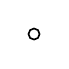
\begin{tikzpicture}
	\node[circle, draw, semithick, inner sep=0pt, minimum size=4pt] (1) at (0,0) {};
	\end{tikzpicture}
}

%----------------------------------------------------------------------------------------
%	TITLE PAGE
%----------------------------------------------------------------------------------------

\setbeamertemplate{title page}{%

	\begin{tikzpicture}[remember picture,overlay]
	
	% Uni logo
	\node[inner sep=0pt] (logo) at (1.1, 3)
	{
\includegraphics[width=.3\textwidth]{images/logo.pdf}};
	
	% Uni pic
	\node[inner sep=0pt] (logo) at (9.175, 1.62)
	{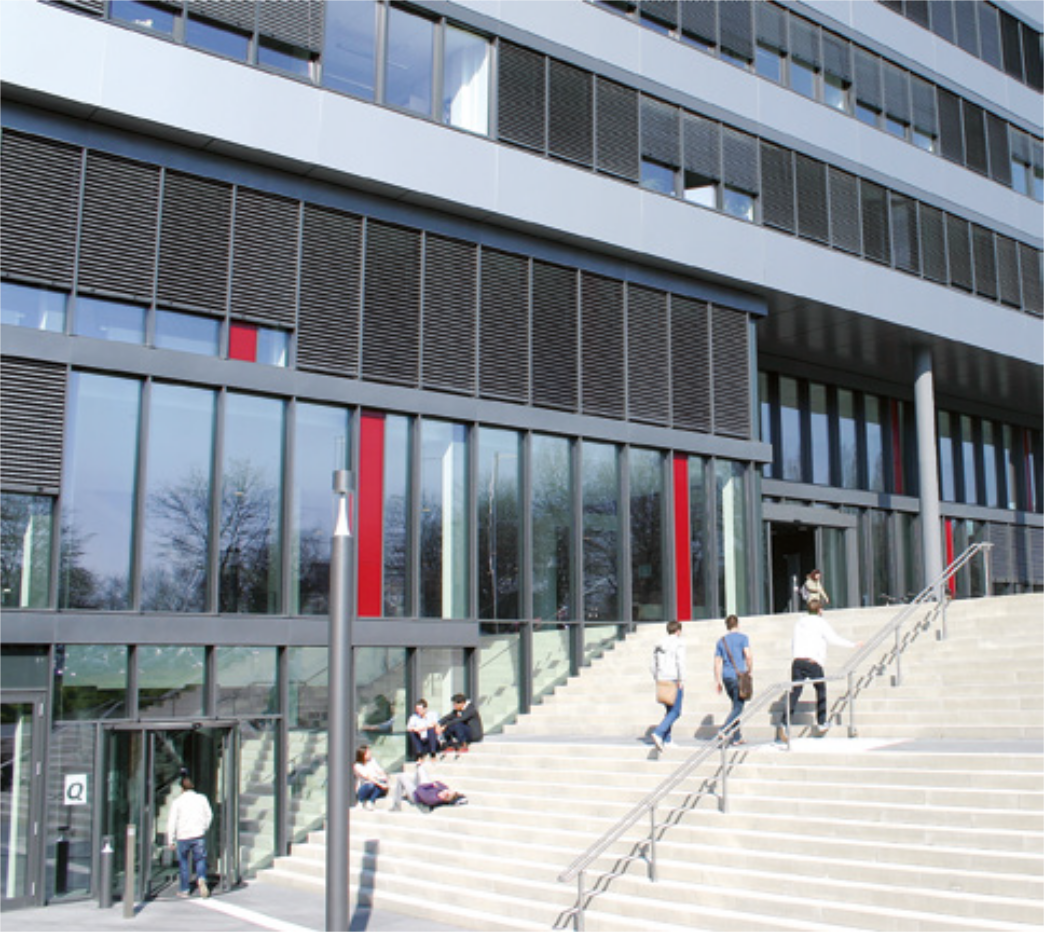
\includegraphics[width=.485\textwidth]{images/unibuilding.png}};
	

	\node[inner sep=0pt] (tit) at (4.40, -2.7)
	{
		\begin{minipage}[t]{1.0\linewidth} 
		\setbeamercolor{title}{bg=\upbcolor,fg=white}	
		
		\begin{minipage}[t]{1.0\linewidth} 
		\setbeamercolor{title}{bg=,fg=uni-blue}	
		\begin{beamercolorbox}[sep=2pt,left]{title}
		{\hspace{4pt}{\vspace{0.1cm}\fontsize{10}{16}\fontfamily{phv}\fontseries{bc}\selectfont\bfseries\insertinstitute}}
		\end{beamercolorbox}
		
		\end{minipage}  	
		
		\begin{minipage}{1.0\linewidth} 
		
		
		\begin{beamercolorbox}[sep=8pt,left]{title}
		
		{\lenitem{\fontsize{\upbtitlesize}{\upbtitlelinespace}\fontfamily{phv}\fontseries{mc}\selectfont\bfseries\color{white}\raggedright\inserttitle}}%
		
		\end{beamercolorbox}
		
		\end{minipage}  	
		
		\ifx\insertsubtitle\@empty%
		\else%
		{		\begin{minipage}[t]{0.9\linewidth} 
			\setbeamercolor{title}{bg=,fg=uni-blue}	
			\begin{beamercolorbox}[sep=4pt,left]{subtitle}
			{\hspace{4pt}\vspace{0.2cm}{\fontsize{10}{16}\fontfamily{phv}\fontseries{bc}\selectfont\bfseries \insertsubtitle}}
			\end{beamercolorbox}
			\end{minipage}  	
		}
		\fi%   			
		
		\end{minipage}  		
		
	};
	
	\end{tikzpicture}	
	
}

%----------------------------------------------------------------------------------------
%	FRAME TITLE THEME
%----------------------------------------------------------------------------------------

\setbeamertemplate{frametitle}
{
	\nointerlineskip
	
	\fontfamily{phv}\fontseries{bc}\selectfont\bfseries 
	\setbeamercolor{frametitle}{bg=,fg=\upbcolor}	
	
	\begin{beamercolorbox}[sep=0.3cm,ht=5.3em,wd=\paperwidth]{frametitle}
		\vbox{}\vskip-2ex%
		\hspace{0.05cm}
		
\includegraphics[width=1.8cm]{images/logo}
		\hfill
		\vskip1.2ex%
		\vspace{0.1cm}
		\hspace{0.0cm}
		\insertframetitle
	\end{beamercolorbox}
	\vspace{-0.4cm}
	
}

% Title
\title{Complex Service Orchestration with OSM and OpenStack} 

% Sub Title
\subtitle{Mini-Project Proposal}

% Your name
\author{Ashwin Prasad Shivarpatna Venkatesh}

% Your institution for the title page
\institute{Future Internet} 

% Date, can be changed to a custom date
\date{\today} 

% Choose primary UPB color for title, headings etc.. 
% Choose from 
% (uni-cyan, uni-black, uni-blue, uni-orange, uni-purple, uni-green)
\newcommand{\upbcolor}{uni-blue} 




%----------------------------------------------------------------------------------------
%	TITLE PAGE
%----------------------------------------------------------------------------------------


\begin{document}

{
\upbtitlebackground 
\begin{frame}
%\upblogo
\titlepage % Print the title page as the first slide
\end{frame}
}


%----------------------------------------------------------------------------------------
%	PRESENTATION SLIDES
%----------------------------------------------------------------------------------------

\begin{frame}
\frametitle{Goals}
\begin{itemize}
	\item Hands-on experiments with tools\\
	\begin{itemize}
		\item Open Source MANO (OSM) / Sonata
		\item OpenStack
		\item Ubuntu Cloud Image
		\item Cloud-init
		\item ...
	\end{itemize} \pause
	\item Build and deploy a complex service in virtual environment\pause
	\item Get \textbf{Servce Function Chaining:} VNF Forwarding Graph to work (?)	
	\begin{itemize}
		\item Currently unstable in OSM, could lead to a pull request
	\end{itemize}

\end{itemize}
\end{frame}


\begin{frame}
\Huge{\centerline{Scenario}}
\end{frame}


\begin{frame}
\begin{onlyenv}<1>
	
	\begin{figure}
		\centering
		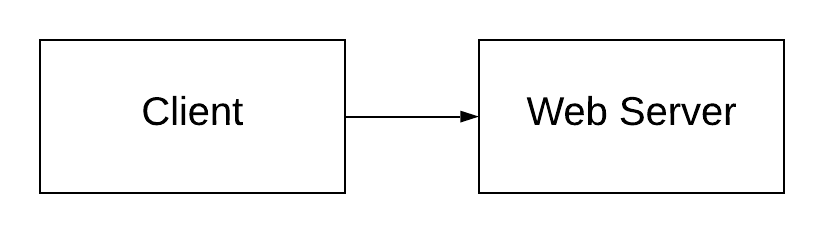
\includegraphics[width=1\linewidth]{images/1}
		\label{fig:1}
	\end{figure}
	
\end{onlyenv}

\begin{onlyenv}<2>
	
	\begin{figure}
		\centering
		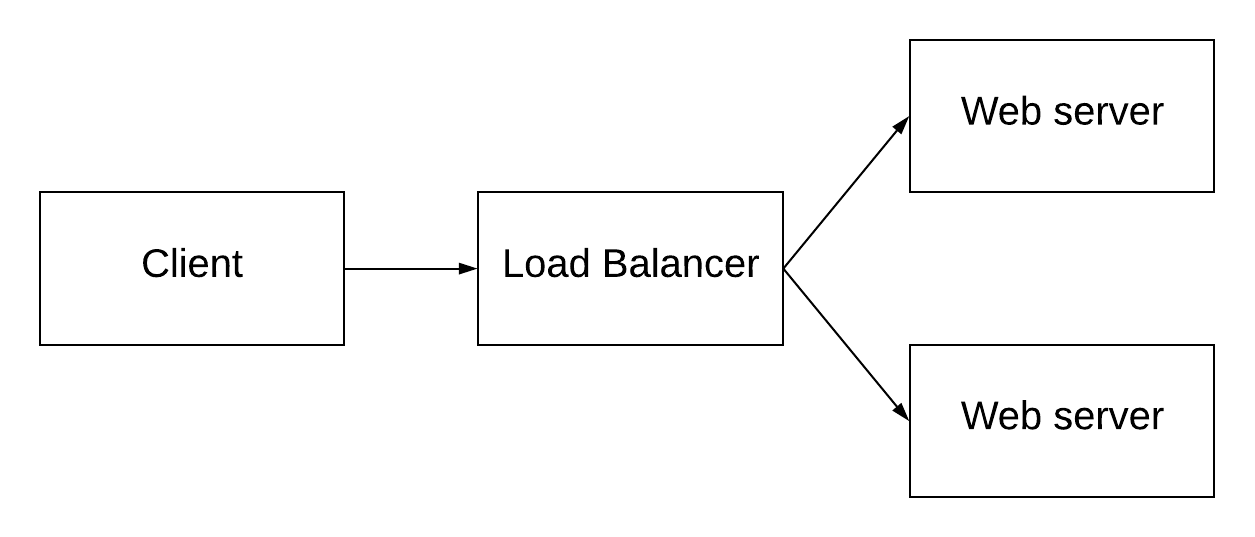
\includegraphics[width=1\linewidth]{images/2}
		\label{fig:2}
	\end{figure}
	
\end{onlyenv}

\begin{onlyenv}<3>
	
	\begin{figure}
		\centering
		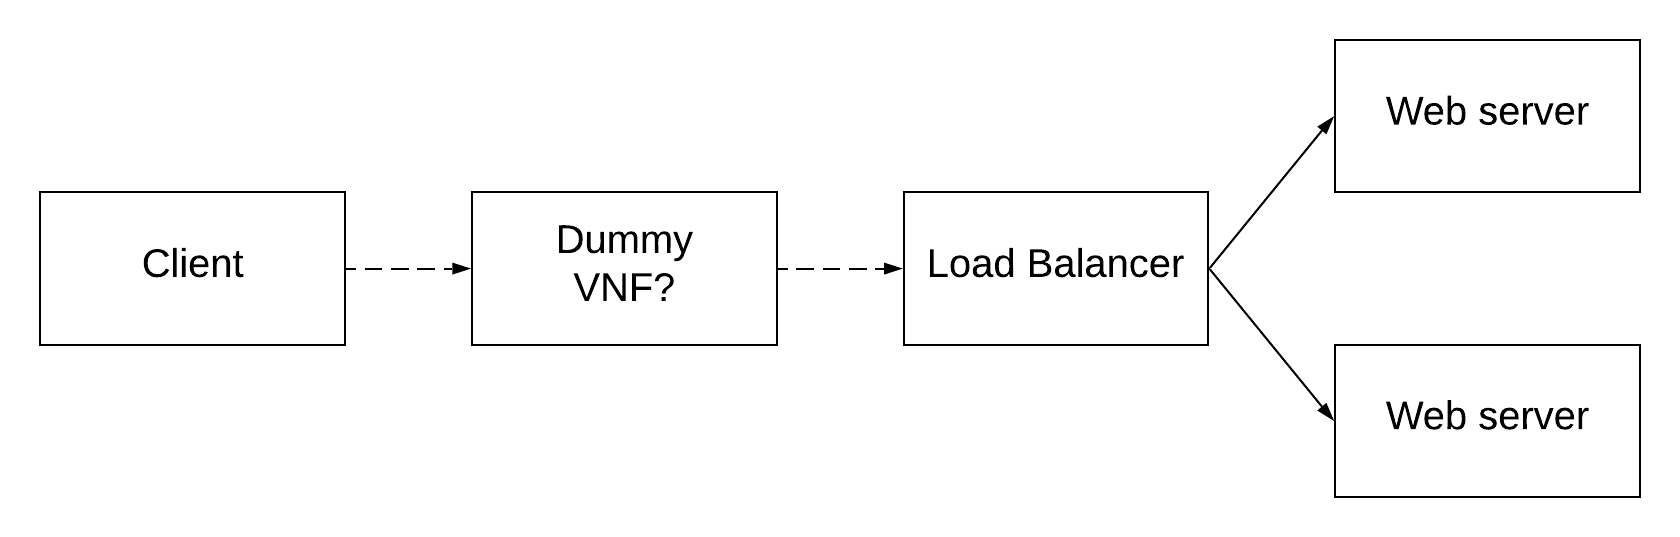
\includegraphics[width=1\linewidth]{images/3}
		\label{fig:3}
	\end{figure}
	
\end{onlyenv}


\end{frame}




%------------------------------------------------

\begin{frame}

\Huge{\centerline{Progress so far...}}

\end{frame}

%----------------------------------------------------------------------------------------

\begin{frame}
\frametitle{Progress so far...}


\begin{enumerate}
	\item \textbf{Environment Setup}\\
	\begin{itemize}
		\item OSM Release 5
		\item DevStack Ocata (OpenStack for dev)
	\end{itemize} \pause

	\item \textbf{Virtual Function Preparation}\\
	\begin{itemize}
		\item Base Image - Ubuntu Cloud Image 16.04
		\item Load Balancer - HAProxy
		\item Web Server - Nginx		
	\end{itemize} \pause

	\item \textbf{Descriptor Creation}\\
	\begin{itemize}
		\item Network Service Descriptor (NSD)
		\item Virtual Network Function Descriptor (VNFD)
		\item OSM provides a tool		
	\end{itemize} \pause
	
\end{enumerate}

\begin{onlyenv}<4>
	
	
	\begin{tikzpicture}[remember picture,overlay]
	\node[drop shadow={shadow xshift=.8ex,shadow yshift=-.8ex},fill=white,draw] at (current page.center) {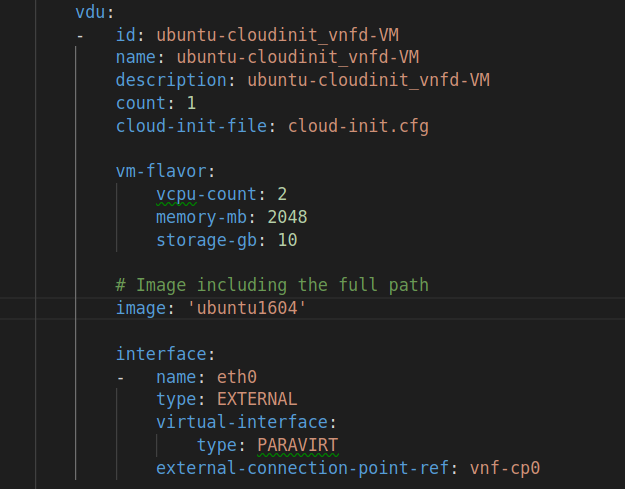
\includegraphics[width=11cm]{images/vnfd-snippet}};
	\end{tikzpicture}
	
\end{onlyenv}

\begin{onlyenv}<5>
	
	
	\begin{tikzpicture}[remember picture,overlay]
	\node[drop shadow={shadow xshift=.8ex,shadow yshift=-.8ex},fill=white,draw] at (current page.center) {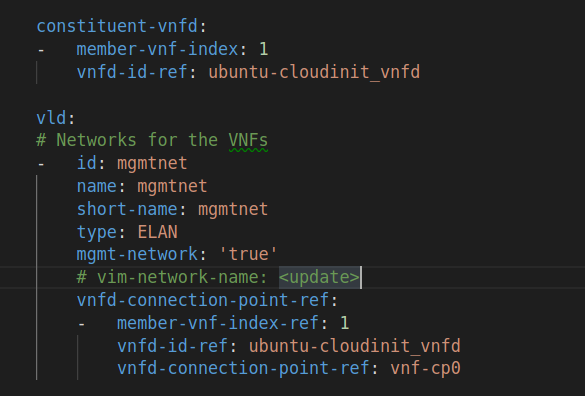
\includegraphics[width=11cm]{images/nsd-snip}};
	\end{tikzpicture}
	
\end{onlyenv}

\end{frame}


\begin{frame}

\Huge{\centerline{What's Left?}}

\end{frame}


\begin{frame}
\frametitle{What's Left?}

\begin{enumerate}
	\item \textbf{Integration | 1 week}\\
	\begin{itemize}
		\item NSD and VNFD
		\item cloud-init scripts
	\end{itemize} \pause

	\item \textbf{Forwarding Graphs | 2 weeks}\\
	\begin{itemize}
		\item Investigate further..
	\end{itemize} \pause
	
	\item \textbf{Testing and Documentation | 1 week}\\
	
\end{enumerate}

\end{frame}

\begin{frame}
\frametitle{GitHub}

\begin{figure}
	\centering
	
\includegraphics[width=0.5\linewidth]{images/gihubqr}
	\label{fig:gihubqr}
\end{figure}

\large{\centerline{\textbf{ashwinprasadme}/Future-Internet-SS19-Mini-Project}}

\end{frame}

\end{document} 